\documentclass[11pt,a4paper]{article}
\usepackage[utf8]{inputenc}
\usepackage[T1]{fontenc}
\usepackage{amsthm} %numéroter les questions
\usepackage[english]{babel}
\usepackage{datetime}
\usepackage{xspace} % typographie IN
\usepackage{hyperref}% hyperliens
\usepackage[all]{hypcap} %lien pointe en haut des figures
\usepackage[french]{varioref} %voir x p y
\usepackage{fancyhdr}% en têtes
%\input cyracc.def
\usepackage[]{graphicx} %include pictures
\usepackage{pgfplots}
\usepackage[]{circuitikz}
\usepackage{ifthen}

\usepackage[top=1.3 in, bottom=1.3 in, left=1.3 in, right=1.3 in]{geometry} % Yeah, that's bad to play with margins
\usepackage[]{pdfpages}

\usepackage[]{attachfile}

\usepackage{float}
\usepackage{subfig}

\usepackage{todonotes} % \missingfigure
\usepackage{gensymb} % \ohm

\usepackage{framed}
\usepackage{xcolor}
\definecolor{commentgreen}{RGB}{2,112,10}
\usepackage{listings}
\lstdefinestyle{CStyle}{
    backgroundcolor=\color{white},   
    commentstyle=\color{commentgreen},
    keywordstyle=\color{blue},
    stringstyle=\color{red},
    basicstyle=\footnotesize,
    breakatwhitespace=false,         
    breaklines=true,                 
    captionpos=b,                    
    keepspaces=true,                 
    numbers=left,                    
    numbersep=5pt,                  
    showspaces=false,                
    showstringspaces=false,
    showtabs=false,                  
    tabsize=2,
    language=C
}


\newdateformat{mydate}{v2.0.1}%hack pour remplacer \THEYEAR


\newboolean{corrige}
\ifx\correction\undefined
\setboolean{corrige}{false}% pas de corrigé
\else
\setboolean{corrige}{true}%corrigé
\fi

%\setboolean{corrige}{false}% pas de corrigé

\newboolean{annexes}
\setboolean{annexes}{true}%annexes
%\setboolean{annexes}{false}% pas de annexes

\definecolor{darkblue}{rgb}{0,0,0.5}

\newboolean{mos}
%\setboolean{mos}{true}%annexes
\setboolean{mos}{false}% pas de annexes

\usepackage{aeguill} %guillemets

%% fancy header & foot
\pagestyle{fancy}
%Numero du TP :
\def \labonumber {Projet -- Part 3}
\lhead{[ELEC-H-310] Choucroute numérique\\ \labonumber}
\rhead{\mydate\today\\ page \thepage}
\chead{\ifthenelse{\boolean{corrige}}{Corrigé}{}}
\cfoot{}
%%

\pdfinfo{
/Author (ULB -- BEAMS)
/Title (\labonumber ELEC-H-310)
/ModDate (D:\pdfdate)
}

\hypersetup{
pdftitle={\labonumber [ELEC-H-310] Choucroute numérique},
pdfauthor={ULB -- BEAMS},
pdfsubject={}
}

\theoremstyle{definition}% questions pas en italique
\newtheorem{Q}{Question}[] % numéroter les questions [section] ou non []

\newcommand{\reponse}[1]{% pour intégrer une réponse : \reponse{texte} : sera inclus si \boolean{corrige}
	\ifthenelse {\boolean{corrige}} {\paragraph{Réponse :} \color{darkblue}   #1\color{black}} {}
 }

\newcommand{\addcontentslinenono}[4]{\addtocontents{#1}{\protect\contentsline{#2}{#3}{#4}{}}}

\date{\vspace{-1.7cm}\mydate\today}
\title{\vspace{-2cm}\labonumber\\ Électronique numérique [ELEC-H-310]\\Conception d'une régulation de refroidissement: \\ interactions avec l'utilisateur\ifthenelse{\boolean{corrige}}{~\\Corrigé}{}}

\title{\vspace{-2cm}\labonumber \\ Digital electronics [ELEC-H-310]\\Design of an automatic fanning system: \\ user interaction\ifthenelse{\boolean{corrige}}{~\\Corrigé}{}}

%\author{\vspace{-1cm}}%\textsc{Yannick Allard}}

\setlength{\parskip}{0.2cm plus2mm minus1mm} %espacement entre §
\setlength{\parindent}{0pt}


















\begin{document}
\pagestyle{empty}
\maketitle
% \vspace*{-1cm}




% ########   ##     ##  ##########  
% ##     ##  ##     ##      ##      
% ##     ##  ##     ##      ##      
% ########   ##     ##      ##      
% ##     ##  ##     ##      ##      
% ##     ##  ##     ##      ##      
% ########    #######       ##      

\section*{Aims}
During three laboratory sessions, you will have to design a small cooling control system based on a propeller fan.
You will also have to be able to interact locally (keyboard) with this system.

During this third lab session, you will add two interaction modes between the fanning control system and the user: either locally with a keyboard, or remotely through a serial port.

At the end of this lab session, you should finish your whole automatic fanning control system.


\section*{Prerequisite}
Before entering in the lab, you have to read the project specifications defined in the document ``Design of an automatic fanning system".



\section*{Objectives}
At the end of this lab session, you'll be able to:
\begin{itemize}
	\item Design and implement a serial connection between two processors and explain how it works.
	\item Make numerous peripheral devices communicate with each other.
\end{itemize}


\newpage





% ########   ##      ##  ##########  ########     #####    
%    ##      ###     ##      ##      ##     ##  ##     ##  
%    ##      ## ##   ##      ##      ##     ##  ##     ##  
%    ##      ##  ##  ##      ##      ########   ##     ##  
%    ##      ##   ## ##      ##      ##   ##    ##     ##  
%    ##      ##     ###      ##      ##    ##   ##     ##  
% ########   ##      ##      ##      ##     ##    #####    


\section{Introduction}
During three laboratory sessions, you will have to design a small automatic fanning system based on a propeller fan.
You will also have to be able to interact locally (keyboard) with this system.

During this lab session, you will first build a way to interact with the keyboard of the extension PCB.
Depending on the input character string, different changes will have to be forecast in the operating of the PCB (ex: change of the fanning speed).

Then, you will ensure than similar changes could be done... remotely!
A PC, connected to the processor through a serial cable, will play the role of the control room allowing you to interact with the processes without being physically present.






%  #######   ##            ###     ##     ##  ########   #########  ########   
% ##     ##  ##           ## ##    ##     ##     ##      ##         ##     ##  
% ##         ##          ##   ##   ##     ##     ##      ##         ##     ##  
% ##         ##         ##     ##  ##     ##     ##      ######     ########   
% ##         ##         #########   ##   ##      ##      ##         ##   ##    
% ##     ##  ##         ##     ##    ## ##       ##      ##         ##    ##   
%  #######   #########  ##     ##     ###     ########   #########  ##     ##  



\section{Keyboard interfacing}
\begin{figure}[H]
\center
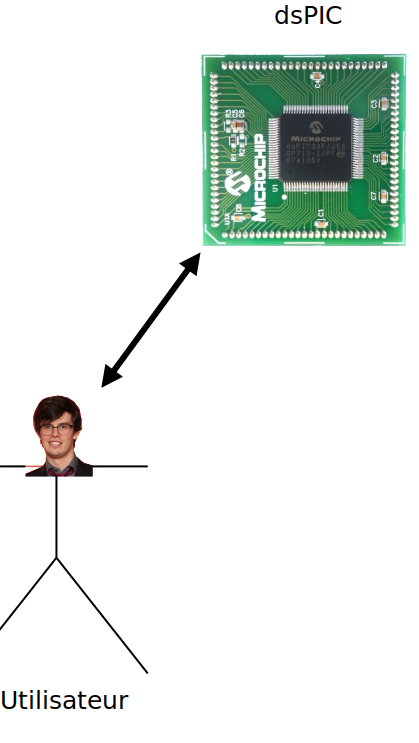
\includegraphics[width=0.5\textwidth]{utilisateur}
\caption{Interaction between the user and the system.}
\label{fig:user}
\end{figure}

As can be seen in the ``Extension PSOC'' file, the keyboard is connected to generic I/O pins of the $\mu$C.
A function allowing to receive the pressed key will be provided (keypad.c and keypad.h files).

\begin{figure}[H]
\center
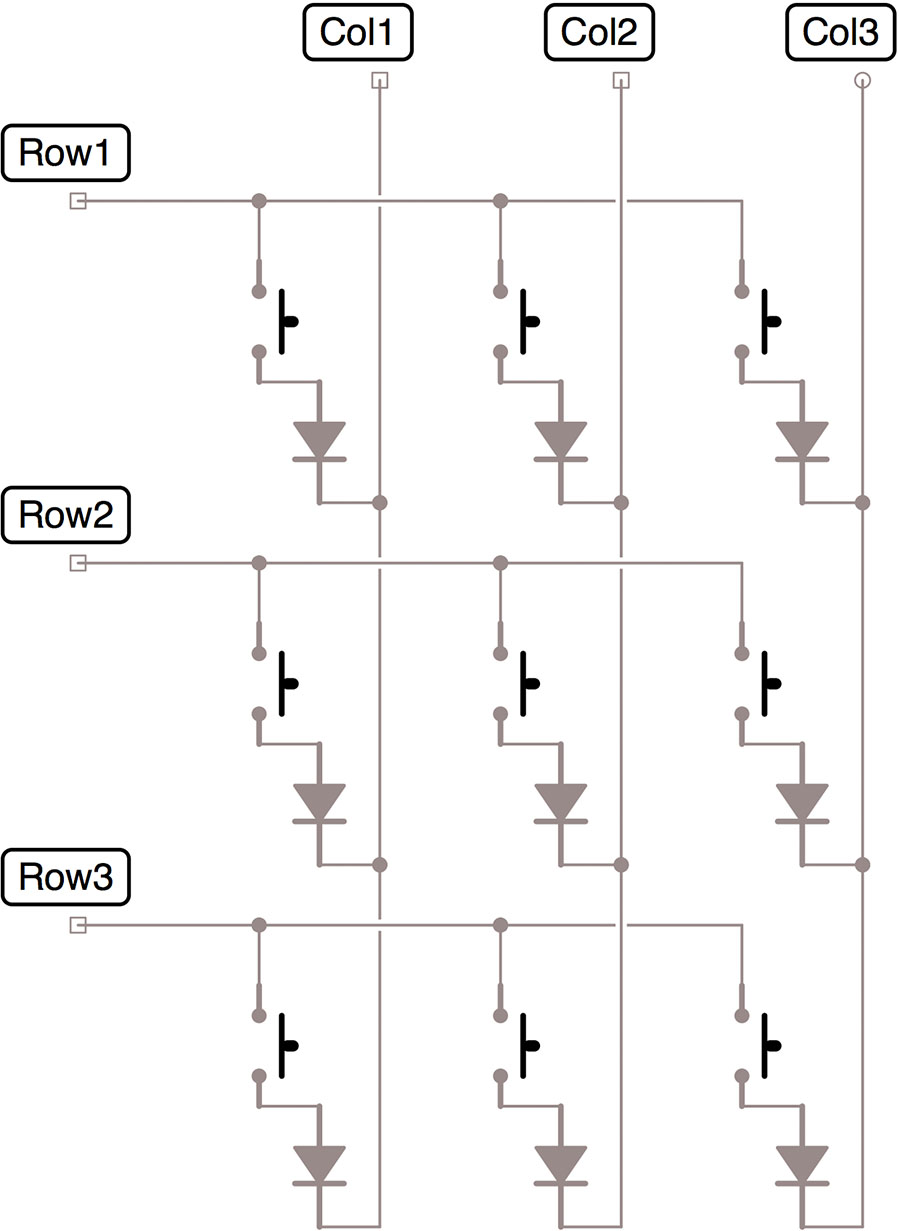
\includegraphics[width=0.4\textwidth]{keyboard_matrix}
\caption{Keyboard matrix for a $3\times 3$ keyboard.}
\label{fig:keyboard_matrix}
\end{figure}

\begin{itemize}
	\item Figure~\ref{fig:keyboard_matrix} shows the electronic diagram of a matrix keyboard. Moreover, a function allowing you to read the pressed key is given on the server (keypad.c and keypad.h files). If the key is effectively pressed, it sends the corresponding character (‘0’ to ‘9’, ‘*’ or ‘\#’).	Otherwise, it sends the value ‘z’. Using the diagram of the matrix keyboard and the code provided, explain how this matrix keyboard works. Are the columns inputs or outputs? Are the rows inputs or outputs? 
	\item In your topDesign.cysch file, instantiate COL1, COL2, COL3, ROW0, ROW1, ROW2 and ROW3 as inputs/outputs appropriately. The inputs should be Digital inputs with ``Resistive pull-up'', the outputs should be digital output with ``Open Drain, Drives low''. 
	\item Add the keypad.h file to the ``Header Files'' folder, and the keypad.c file to the ``Source Files'' folder. Finally, add the following line at the beginning of your firmware code (i.e. the main.c file): 
\begin{lstlisting}[style=CStyle]
#include "keypad.h"	
\end{lstlisting}
\end{itemize}

Now that the keyboard is working, you can write the function allowing to modify the behaviour of your fanning control center depending on which keys are pressed.
The list of the possible commands is given in the global project specifications.
\begin{itemize}
	\item The function allowing you to read the pressed keys requires a large amount of instructions.
	Where do you have to call this function in order to avoid blocking the processor uselessly?
	\item When the user is typing on the keyboard, the LCD has to display the pressed key.
	Once the command is fully entered, the LCD has to display the voltage of the light sensor again.
\end{itemize}







%  #######   #########  ########   ########   #########  
% ##     ##  ##         ##     ##     ##      ##         
% ##         ##         ##     ##     ##      ##         
%  #######   ######     ########      ##      ######     
%        ##  ##         ##   ##       ##      ##         
% ##     ##  ##         ##    ##      ##      ##         
%  #######   #########  ##     ##  ########   #########  


\section{Serial connection}
In this part, you will send and receive data to/from the PC through the serial port in order to follow the evolution of the voltage of the light sensor, as well as to receive the commands from the PC to adjust the fan speed.

The last module to set is the serial port, allowing to communicate remotely with a PC.
This module is named UART (Universal Asynchronous Receiver / Transmitter).

Before designing this communication, you will have to set the PSOC and the PC in order to make them ``speak the same language".
We will start by the PSOC setup. Add an UART component to the topDesign.cysch file. Connect the \texttt{RX} and the \texttt{TX} ports of the UART component to one of the GPIO ports on the PSOC extension board. Double-click on the UART component to set the UART communication parameters.

The parameters of the UART connection are the following: 
\begin{itemize}
	\item Baudrate: 9600
	\item Data bits: 8
	\item No parity bit
	\item Only one stop bit
	\item No flow control
\end{itemize}

\subsection{Sending data to the PC}
To send and receive the data on the PC side, use the software ``Termite 3.4'' that you can find on the server. This software allows to connect an USB-to-serial converter to the PC and exchange data with an UART device. Make sure the UART communication parameters match those of the PSOC. To determine the correct COM port, connect the USB-to-serial converter to the PC and do the following : 
\begin{itemize}
\item Wait for Windows to install the drivers
\item Open the Device Manager by pressing the Windows Key $+$ R. Type “devmgmt.msc” and press Enter.
\item Expand the Ports (COM \& LPT) section.
\item Find the COM port associated to the USB-to-serial converter. 
\end{itemize}
Connect the USB-to-serial converter between the PC and the PSOC (\textbf{note that the PSOC \texttt{TX} port corresponds to the USB-to-serial \texttt{RX} port, and vice-versa}). Do not forget to connect the ground of the PSOC to the ground of the USB-to-serial converter. 

To send data to the PC from the PSOC device, refer to the UART datasheet. The following tasks need to be performed: 
\begin{itemize}
	\item Start the UART transceiver. 
	\item Test the UART transmission by sending a string with the \texttt{UART\_PutString} function and check on Termite if you received it correctly.
	\item Send specific data over the UART by using \texttt{UART\_PutChar()} for only one character, or \texttt{UART\_PutString()} for several at once.
    To convert a string into ASCII characters, use the function \texttt{sprintf}:
    % To convert an (single-digit) integer to a ASCII character, you can just add the term '0' (see code snippet below)
\begin{lstlisting}[style=CStyle]
char tab[2];
int value = 42;
sprintf(tab, "%d", value);
\end{lstlisting}
Note that you can't convert \texttt{float} variables.
\end{itemize}





\subsection{Sending commands from the PC}

We want the PSOC to trigger an interrupt each time a byte is received from the PC on the UART port. To do this:
\begin{itemize}
	\item Check the ``\texttt{RX} - on byte received'' box in the UART component in your topDesign.cysch file.
	\item Add an ``Interrupt'' component connected to the \texttt{rx\_interrupt} input in the topDesign.cysch file.
	\item In the firmware (i.e. main.c file), don't forget to start the interrupt related to the UART reception.
	\item Write the code for the UART ISR, based on the sample code below: 
\end{itemize}


%% USE LSTLISTINGS package
\begin{lstlisting}[style=CStyle]
CY_ISR ( isr_uart_rx_Handler ) {
    uint8_t status = 0;
    do{
        // Checks if no UART Rx errors
        status = UART_ReadRxStatus();
        if ((status & UART_RX_STS_PAR_ERROR) | 
            (status & UART_RX_STS_STOP_ERROR) | 
            (status & UART_RX_STS_BREAK) | 
            (status & UART_RX_STS_OVERRUN) ) {
            // Parity, framing, break or overrun error
            LCD_Position(1,0);
            LCD_PrintString("UART err");
        }
        // Check that rx buffer is not empty and get rx data
        if ( (status & UART_RX_STS_FIFO_NOTEMPTY) != 0){
            
            rxData = UART_ReadRxData();
            // Here comes your code, ...
            // ... what do you do with rxData ? 
        }
    }while ((status & UART_RX_STS_FIFO_NOTEMPTY) != 0);    
}
\end{lstlisting}



%  #######   ##     ##   #######   ##########    #####    ##       ##  
% ##     ##  ##     ##  ##     ##      ##      ##     ##  ###     ###  
% ##         ##     ##  ##             ##      ##     ##  ## ## ## ##  
% ##         ##     ##   #######       ##      ##     ##  ##  ###  ##  
% ##         ##     ##         ##      ##      ##     ##  ##       ##  
% ##     ##  ##     ##  ##     ##      ##      ##     ##  ##       ##  
%  #######    #######    #######       ##        #####    ##       ##  



\section{Project customization}
Your fanning control system is now functional, you can add different features to enhance it!


\end{document}
